% Options for packages loaded elsewhere
% Options for packages loaded elsewhere
\PassOptionsToPackage{unicode}{hyperref}
\PassOptionsToPackage{hyphens}{url}
\PassOptionsToPackage{dvipsnames,svgnames,x11names}{xcolor}
%
\documentclass[
  english,
  11pt,
]{article}
\usepackage{xcolor}
\usepackage[margin=2.5cm]{geometry}
\usepackage{amsmath,amssymb}
\setcounter{secnumdepth}{3}
\usepackage{iftex}
\ifPDFTeX
  \usepackage[T1]{fontenc}
  \usepackage[utf8]{inputenc}
  \usepackage{textcomp} % provide euro and other symbols
\else % if luatex or xetex
  \usepackage{unicode-math} % this also loads fontspec
  \defaultfontfeatures{Scale=MatchLowercase}
  \defaultfontfeatures[\rmfamily]{Ligatures=TeX,Scale=1}
\fi
\usepackage{lmodern}
\ifPDFTeX\else
  % xetex/luatex font selection
\fi
% Use upquote if available, for straight quotes in verbatim environments
\IfFileExists{upquote.sty}{\usepackage{upquote}}{}
\IfFileExists{microtype.sty}{% use microtype if available
  \usepackage[]{microtype}
  \UseMicrotypeSet[protrusion]{basicmath} % disable protrusion for tt fonts
}{}
\makeatletter
\@ifundefined{KOMAClassName}{% if non-KOMA class
  \IfFileExists{parskip.sty}{%
    \usepackage{parskip}
  }{% else
    \setlength{\parindent}{0pt}
    \setlength{\parskip}{6pt plus 2pt minus 1pt}}
}{% if KOMA class
  \KOMAoptions{parskip=half}}
\makeatother
% Make \paragraph and \subparagraph free-standing
\makeatletter
\ifx\paragraph\undefined\else
  \let\oldparagraph\paragraph
  \renewcommand{\paragraph}{
    \@ifstar
      \xxxParagraphStar
      \xxxParagraphNoStar
  }
  \newcommand{\xxxParagraphStar}[1]{\oldparagraph*{#1}\mbox{}}
  \newcommand{\xxxParagraphNoStar}[1]{\oldparagraph{#1}\mbox{}}
\fi
\ifx\subparagraph\undefined\else
  \let\oldsubparagraph\subparagraph
  \renewcommand{\subparagraph}{
    \@ifstar
      \xxxSubParagraphStar
      \xxxSubParagraphNoStar
  }
  \newcommand{\xxxSubParagraphStar}[1]{\oldsubparagraph*{#1}\mbox{}}
  \newcommand{\xxxSubParagraphNoStar}[1]{\oldsubparagraph{#1}\mbox{}}
\fi
\makeatother


\usepackage{longtable,booktabs,array}
\newcounter{none} % for unnumbered tables
\usepackage{calc} % for calculating minipage widths
% Correct order of tables after \paragraph or \subparagraph
\usepackage{etoolbox}
\makeatletter
\patchcmd\longtable{\par}{\if@noskipsec\mbox{}\fi\par}{}{}
\makeatother
% Allow footnotes in longtable head/foot
\IfFileExists{footnotehyper.sty}{\usepackage{footnotehyper}}{\usepackage{footnote}}
\makesavenoteenv{longtable}
\usepackage{graphicx}
\makeatletter
\newsavebox\pandoc@box
\newcommand*\pandocbounded[1]{% scales image to fit in text height/width
  \sbox\pandoc@box{#1}%
  \Gscale@div\@tempa{\textheight}{\dimexpr\ht\pandoc@box+\dp\pandoc@box\relax}%
  \Gscale@div\@tempb{\linewidth}{\wd\pandoc@box}%
  \ifdim\@tempb\p@<\@tempa\p@\let\@tempa\@tempb\fi% select the smaller of both
  \ifdim\@tempa\p@<\p@\scalebox{\@tempa}{\usebox\pandoc@box}%
  \else\usebox{\pandoc@box}%
  \fi%
}
% Set default figure placement to htbp
\def\fps@figure{htbp}
\makeatother



\ifLuaTeX
\usepackage[bidi=basic,shorthands=off]{babel}
\else
\usepackage[bidi=default,shorthands=off]{babel}
\fi
\ifLuaTeX
  \usepackage{selnolig} % disable illegal ligatures
\fi


\setlength{\emergencystretch}{3em} % prevent overfull lines

\providecommand{\tightlist}{%
  \setlength{\itemsep}{0pt}\setlength{\parskip}{0pt}}



 


\renewcommand{\and}{\par}
\setlength{\headheight}{30pt}
\usepackage{graphicx}
\usepackage{xcolor}
\usepackage{float}
\usepackage{placeins}
\usepackage{longtable}
\usepackage{caption}
\usepackage{fancyhdr}
\usepackage{needspace}
\usepackage{array}
\usepackage{amsmath}
\renewcommand{\headrulewidth}{0pt}

\raggedbottom
\captionsetup[figure]{skip=2pt}
\newcommand{\legendfont}{\fontsize{10pt}{10pt}\bfseries\selectfont}
\newcommand{\resetfont}{\normalsize\normalfont}

%  Väljer språk för automatiska titlar -->

% \selectlanguage{english}

%  Byter språket på figur- och tabellbeskrivningar till angivna namn

\captionsetup[table]{name = Table}
\setcounter{table}{0}
\captionsetup[figure]{name = Figure}
\setcounter{figure}{0}

%  Anger att tabellbeskrivningar hamnar ovanför tabellen

\floatstyle{plaintop}
\restylefloat{table}

%  Anger sidnumreringens position

\fancyhf{}
\fancyfoot[C]{\thepage}
\pagestyle{fancy}

\fancyhead[L]{\itshape\footnotesize{732A99 Machine Learning - Lab Report}}
\fancyhead[R]{\itshape\footnotesize{jonda228, jonha849, kerar739}}

% lot and lof
\usepackage{etoolbox}
\pretocmd{\listoffigures}{\clearpage}{}{}
\apptocmd{\listoftables}{\clearpage}{}{}

\setcounter{secnumdepth}{3}
\setcounter{tocdepth}{3}
\setlength{\parskip}{\smallskipamount}
\setlength{\parindent}{0pt}

% \usepackage{titlesec}
% \titleformat{\chapter}
%    {\normalfont\LARGE\bfseries}{\thechapter.}{1em}{}
% \titlespacing{\chapter}{0pt}{50pt}{2\baselineskip}

\usepackage{ragged2e}

% custom command for thesis front page + 1
\newcommand{\makereportfrontpage}{
\begin{titlepage}
\clearpage\thispagestyle{empty}
\centering
\vspace{2cm}

{\large Master's Programme in Statistics and Machine Learning \par}
\vspace{4cm}
{\Huge 732A99 Machine Learning\par}
\vspace{1cm}
{\Huge Computer Lab 1 Block 1\par}
\vspace{1cm}
{\Huge Lab Report \par}


\vspace{2cm}

{\normalsize Jonas Danielsson \\ jonda228 \par}
{\normalsize Jonas Hautamäki Bengtsson \\ jonha849 \par}
{\normalsize Kerstin Arbring \\ kerar739 \par}
\vspace{3cm}


\includegraphics[scale=0.75]{liu_logga.png}

\vfill

{\normalsize
Division of Statistics and Machine Learning\\
Department of Computer and Information Science\\
Linköping University\\
\today\par}

\end{titlepage}

% \clearpage
% \thispagestyle{empty}
% \vspace*{\fill}
%
% \clearpage
% \setcounter{page}{1}
}
\makeatletter
\@ifpackageloaded{caption}{}{\usepackage{caption}}
\AtBeginDocument{%
\ifdefined\contentsname
  \renewcommand*\contentsname{Table of contents}
\else
  \newcommand\contentsname{Table of contents}
\fi
\ifdefined\listfigurename
  \renewcommand*\listfigurename{List of Figures}
\else
  \newcommand\listfigurename{List of Figures}
\fi
\ifdefined\listtablename
  \renewcommand*\listtablename{List of Tables}
\else
  \newcommand\listtablename{List of Tables}
\fi
\ifdefined\figurename
  \renewcommand*\figurename{Figure}
\else
  \newcommand\figurename{Figure}
\fi
\ifdefined\tablename
  \renewcommand*\tablename{Table}
\else
  \newcommand\tablename{Table}
\fi
}
\@ifpackageloaded{float}{}{\usepackage{float}}
\floatstyle{ruled}
\@ifundefined{c@chapter}{\newfloat{codelisting}{h}{lop}}{\newfloat{codelisting}{h}{lop}[chapter]}
\floatname{codelisting}{Listing}
\newcommand*\listoflistings{\listof{codelisting}{List of Listings}}
\makeatother
\makeatletter
\makeatother
\makeatletter
\@ifpackageloaded{caption}{}{\usepackage{caption}}
\@ifpackageloaded{subcaption}{}{\usepackage{subcaption}}
\makeatother
\usepackage{bookmark}
\IfFileExists{xurl.sty}{\usepackage{xurl}}{} % add URL line breaks if available
\urlstyle{same}
% fallback for those not using the hyperref driver hyperxmp:
\makeatletter
\@ifundefined{xmpquote}{\newcommand{\xmpquote}[1]{#1}}{}
\makeatother
\hypersetup{
  pdflang={en},
  colorlinks=true,
  linkcolor={blue},
  filecolor={Maroon},
  citecolor={Blue},
  urlcolor={Blue},
  pdfcreator={LaTeX via pandoc}}


\author{}
\date{}
\begin{document}


\section{Assignment 3 - Logistic regression and Basis Function
Expansion}\label{assignment-3---logistic-regression-and-basis-function-expansion}

Visualization of the data shows that there are values equal to zero in
the measures, including plasma glucose which is one of the predictors of
interest in this assignment. \texttt{Glucose\ ==\ 0} is not a feasible
value, but rather representing a missing value. All cases (n=5) with
plasma glucose equal to zero were excluded from the data before the
regression analysis.

\subsection{Scatterplot diabetes vs
age}\label{scatterplot-diabetes-vs-age}

\pandocbounded{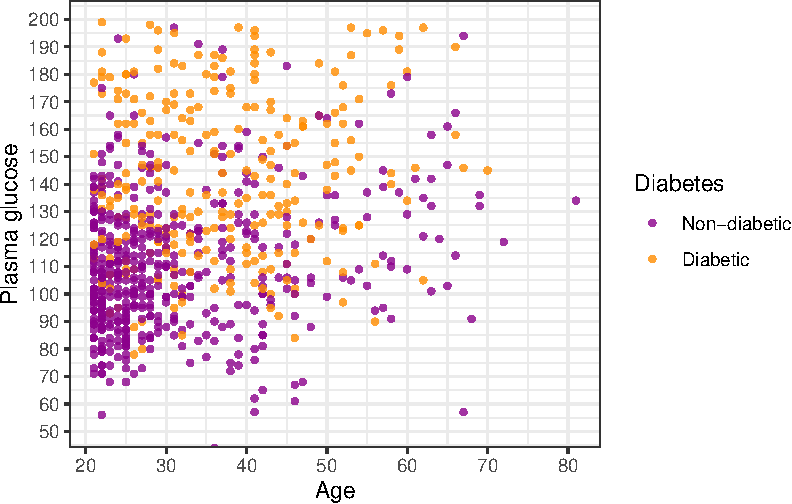
\includegraphics[keepaspectratio]{lab1_assignment3_files/figure-pdf/unnamed-chunk-2-1.pdf}}

Plotting plasma glucose levels vs.~age shows that the two response
groups, \texttt{Non-diabetic} and \texttt{Diabetic}, show a substantial
overlap. \texttt{Diabetes} would therefore not be easily predicted by
\texttt{Age} and \texttt{Glucose} in a standard logistic regression
model which would not be able to derive a straight line clearly
separating the groups.

\subsection{Logistic regression model}\label{logistic-regression-model}

The vector form of the probailistic equation for a logistic regression
model is \begin{equation}\protect\phantomsection\label{eq-logistic}{
P(Y = 1 \mid \mathbf{x}) = \operatorname{sigmoid}(\boldsymbol{\theta}^{T}\mathbf{x})
}\end{equation} where the sigmoid function is
\begin{equation}\protect\phantomsection\label{eq-sigmoid}{
\mathit{sigmoid}(\boldsymbol{\theta}^{T}\mathbf{x}) = \frac{1}{1 + e^{-\boldsymbol{\theta}^{T}\mathbf{x}}}
}\end{equation}

For \texttt{Diabetes} as the binary target/response (y), and
\texttt{Glucose} and \texttt{Age} as features/predictors (x1, x2):

\begin{equation}\protect\phantomsection\label{eq-logistic-expanded}{
P(Y = 1 \mid x_1, x_2) = \frac{1}{1 + e^{-(\theta_0 + \theta_1 x_1 + \theta_2 x_2)}}
}\end{equation} Training a logistic regression model on the (entire)
provided data set, using glm() in R, results in the following
coefficients

\[
\theta_0 = -6.2252\\
\theta_1 = 0.0384\\
\theta_2 = 0.0231\\
\] and the corresponding probabilistic equation

\begin{equation}\protect\phantomsection\label{eq-logistic-fitted}{
P(Y=1 \mid x_1,x_2) =
\frac{1}{1 + e^{-(
-6.2252 +
0.0384x_1 +
0.0231x_2)}}
}\end{equation}

The training misclassification error for this model is 0.26.

\subsection{Scatterplot colored by
predicions}\label{scatterplot-colored-by-predicions}

\pandocbounded{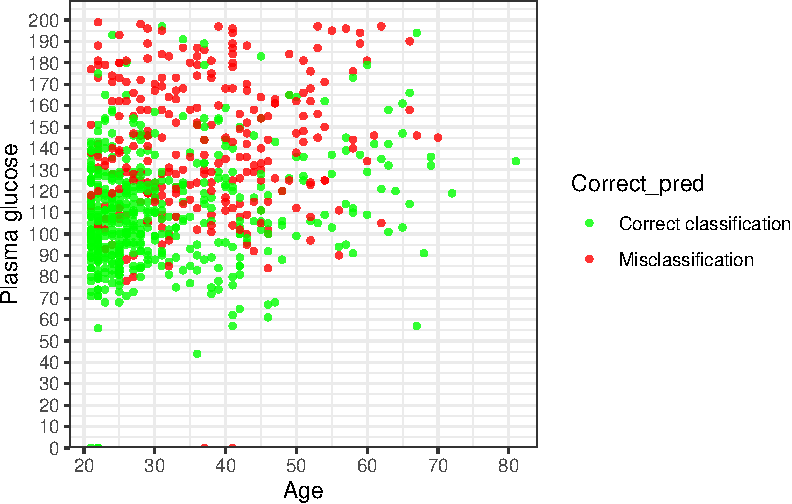
\includegraphics[keepaspectratio]{lab1_assignment3_files/figure-pdf/unnamed-chunk-3-1.pdf}}

\subsection{Decision boundary
equation}\label{decision-boundary-equation}

Setting the probabilistic equation in Equation~\ref{eq-logistic-fitted}
equal to \texttt{r} (here \texttt{=\ 0.5}) gives the approximate
decision boundary equation as \[
-6.2252 +
0.0384x_1 +
0.0231x_2 = 0
\] i.e., \[
-6.2252 +
0.0384Glucose +
0.0231Age = 0
\]

Solving this for \texttt{Glucose} gives the linear decision boundary
line

\begin{equation}\protect\phantomsection\label{eq-glucose}{
\mathit{Glucose} = -\frac{\theta_0 + \theta_2 \mathit{Age}}{\theta_1}
}\end{equation}

approximately

\[
\mathit{Glucose} = - -161.97 - 0.6Age
\] \#\# Scatterplot with decision boundary line for r = 0.5

\pandocbounded{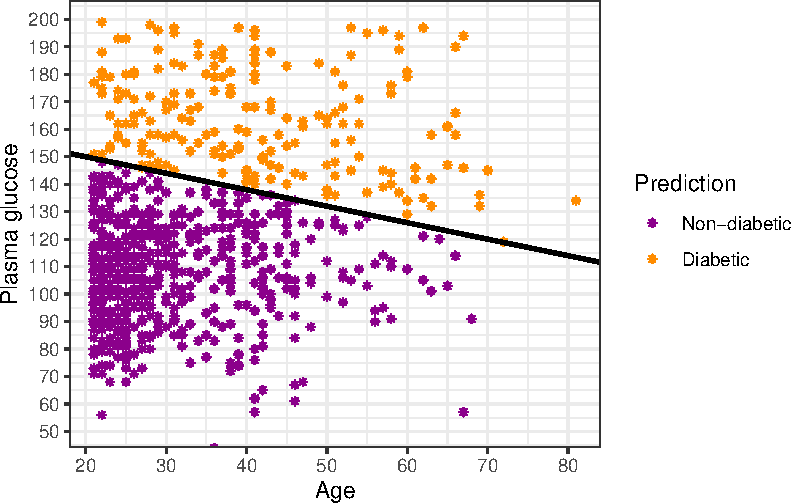
\includegraphics[keepaspectratio]{lab1_assignment3_files/figure-pdf/unnamed-chunk-4-1.pdf}}

\subsection{Scatterplot with decision boundary line for r = 0.2 and r =
0.8}\label{scatterplot-with-decision-boundary-line-for-r-0.2-and-r-0.8}

The equation for the decision boundary line can generically be expressed
as

\begin{equation}\protect\phantomsection\label{eq-boundary-generic}{
x_1 = \frac{\log\left(\frac{r}{1-r}\right) - \theta_0}{\theta_1} - \frac{\theta_2}{\theta_1}x_2
}\end{equation}

which means the intercept changes with r, the slope does not.

With r = 0.2 are more individuals predicted to be diabetic, with r
increased to 0.8 instead fewer individuals. The training
misclassification errors are 0.36 and 0.31 resepectively for the 0.2 and
0.8 cases, both higher than for the 0.5 cutoff case.

\begin{figure}

\begin{minipage}[t]{0.50\linewidth}

\raisebox{-\height}{

\pandocbounded{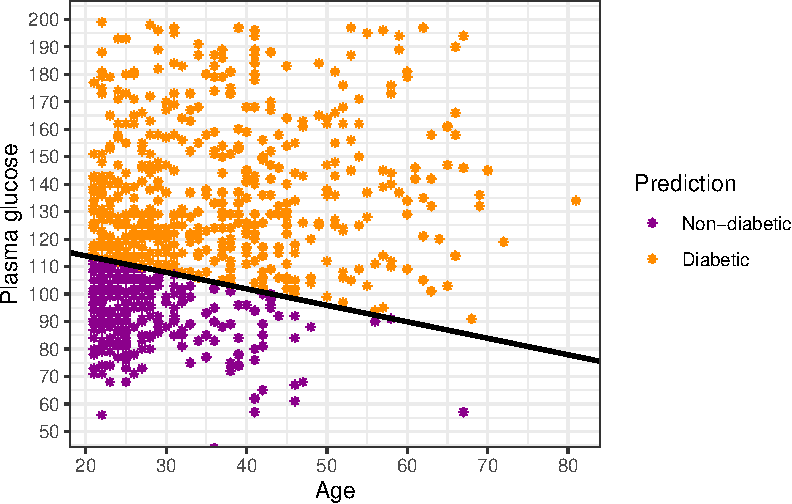
\includegraphics[keepaspectratio]{lab1_assignment3_files/figure-pdf/unnamed-chunk-5-1.pdf}}

}

\end{minipage}%
%
\begin{minipage}[t]{0.50\linewidth}

\raisebox{-\height}{

\pandocbounded{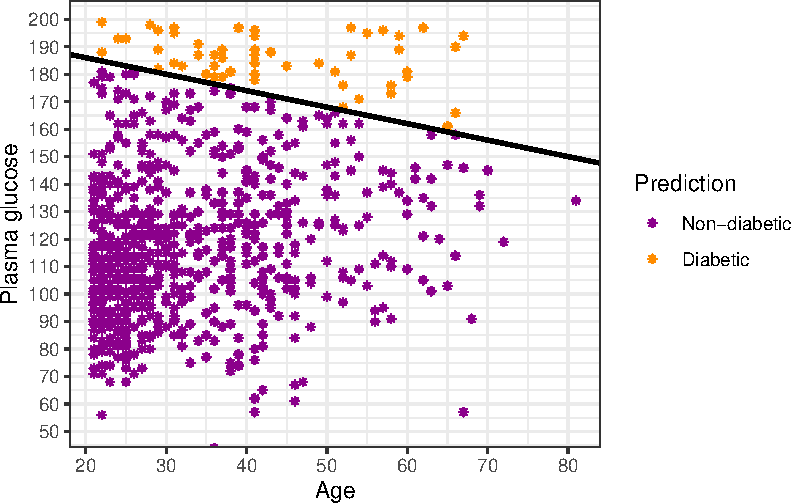
\includegraphics[keepaspectratio]{lab1_assignment3_files/figure-pdf/unnamed-chunk-5-2.pdf}}

}

\end{minipage}%

\end{figure}%




\end{document}
